\chapter{Operazioni preliminari}\label{ch:th-music}

\section{Disclaimer}
Gli autori non sono musicisti, ne hanno mai studiato musica! \\
La nostra conoscenza in merito è stata costruita nel periodo del progetto e come tale potrà contenere inesattezze di ogni sorta.

\section{Dataset}
Il dataset utilizzato è composto da 382 corali composti da Johann Sebastian Bach in formato testuale come mostrato in figura \ref{music-notation}.
\begin{figure}[H]
	\caption{Struttura musicale del corale 10}
	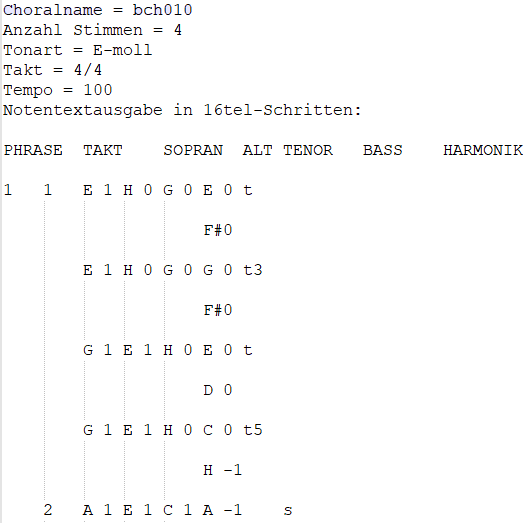
\includegraphics{figures/music-notation.png}
	\label{music-notation}
\end{figure}
\noindent
Dall'header estraiamo alcune informazioni importanti come:
\begin{itemize}
\item Tonart: rappresenta la tonalità con cui è composto il corale (dur = Maggiore, moll = Minore)
\item Takt: rappresenta la time signature del corale
\item Tempo: rappresenta la velocità del corale
\end{itemize}
In particolare la notazione utilizzata per descrivere la tonalità è quella utilizzata principalmente nelle zone di influenza germanica, la conversione ad un sistema a noi più familiare è immediata
\begin{table}[H]
\centering
\begin{tabular}{|l|l|l|l|l|l|l|}
\hline
A  & H  & C  & D  & E   & F  & G  \\ \hline
Do & Re & Mi & Fa & Sol & La & Si \\ \hline
\end{tabular}
\end{table}
\noindent
La composizione vera e propria si articola su diverse colonne:
\begin{itemize}
\item Il numero contenuto nella prima colonna rappresenta l'inizio di una frase (unità musicale che ha senso anche se suonata singolarmente)
\item Il numero contenuto nella seconda colonna rappresenta l'inizio di una nuova battuta
\item La terza colonna rappresenta la nota eseguita dal soprano
\item La quarta colonna rappresenta la nota eseguita dal contralto
\item La quinta colonna rappresenta la nota eseguita dal tenore
\item La sesta colonna rappresenta la nota eseguita dal basso
\item L'ultima colonna ci da un'indicazione riguardo la funzione armonica di una certa battuta.
\end{itemize}
\noindent
Il dataset viene inizialmente suddiviso in corali in tonalità maggiore e corali in tonalità minore in quanto la loro composizione è nettamente diversa.

\section{Preprocessing}
Il dataset così definito è ovviamente impossibile da utilizzare per addestrare un HMM, è necessario, per ogni file, costruire una coppia [stato nascosto-stato visibile] che sia in grado di rappresentarne la struttura musicale. \\
Questa operazione viene effettuata tramite lo script hmm-data.py, che legge i corali e costruisce l'input per il modello di Markov.
In particolare gli stati visibili rappresentano le note relative al soprano, mentre gli stati nascosti rappresentano le corde e la loro relativa funzione armonica. \\
Per ogni corale in ingresso viene prodotto un file con lo stesso nome contenente una serie di coppie di indici come mostrato in figura \ref{data-out}.
\begin{figure}[H]
	\centering
	\caption{Esempio di file processato}
	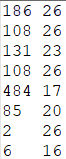
\includegraphics{figures/data-out.png}
	\label{data-out}
\end{figure}
\noindent
Queste coppie di indici fanno riferimento rispettivamente agli stati nascosti e a quelli visibili contenuti nei file "SYMBOLS\_HIDDEN" e "SYMBOLS\_VISIBLE".
Come vediamo dalla figura \ref{hid-vis} (a) uno stato nascosto è nella forma a:b:c:0/Y, dove a rappresenta il numero di semitoni in più del soprano rispetto al basso, in maniera equivalente b e c rappresentano il numero di semitoni in più di contralto e tenore rispetto al basso. \\
In figura \ref{hid-vis} (b) vediamo invece come gli stati visibili siano semplicemente le note della melodia del soprano.
\begin{figure}[H]
	\centering
	\caption{(a) Inizio del file SYMBOLS\_HIDDEN, (b) Inizio del file SYMBOLS\_VISIBLE}
	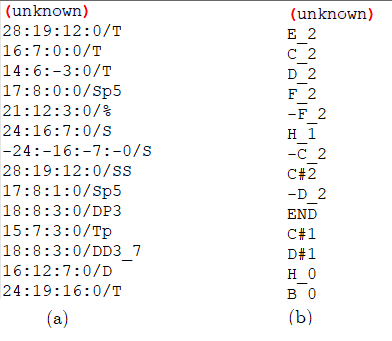
\includegraphics{figures/hid-vis.png}
	\label{hid-vis}
\end{figure}

